\documentclass[a4paper,italian,twoside,openright,11pt]{book}
\usepackage{lipsum} % this is for dummy text
\usepackage{cmap} % makes PDF searchable
\usepackage{babel}
\usepackage{tabulary}
%\usepackage[latin9]{inputenc}
\usepackage[latin1]{inputenc}
\usepackage{lmodern} % Latin Modern font
\usepackage[T1]{fontenc}
\usepackage{textcomp} % needed for fontenc
\usepackage{styles/extref}
	\newcommand{\sectionname}{Sezione}
	\newcommand{\subsectionname}{Sezione}
\usepackage[bookmarksnumbered,final]{styles/easyoutput}
\usepackage{url}
\usepackage[final]{listings}
	\lstset{numbers=left,breaklines}
	\usepackage{acronym}
\usepackage{makeidx}
	\makeindex
%\usepackage[square]{natbib}
\usepackage[binding=0.8cm]{styles/layaureo} % better handling of A4 format
\usepackage{tocbibind} 
\usepackage[labelfont=bf]{caption}[2004/07/16] % format of captions
\usepackage{subfig}
% tables
\usepackage{booktabs}
\usepackage{tabulary}
% citations at the beginning of each chapter
\usepackage{epigraph}
	\setlength{\epigraphwidth}{.59\textwidth}
	\renewcommand{\epigraphsize}{\small}
	\renewcommand{\epigraphflush}{flushleft}
\usepackage{styles/reallyblank} % insert empty page at the beginning of a chapter with empty headings
% the following is for thesis in Italian language; adapt it for English ones
\usepackage{sistyle}
\AddToSIstyle{Italian}{
   \SIdecimalsign{,}
   \SIthousandsep{\,}
   \SIproductsign{\cdot}
   \SIunitsep{\,}
   \SIunitspace{\,}
   \SIunitdot{\cdot}
   \SIobeyboldfalse
   \SIgroupfourfalse}
\SIstyle{Italian}
\usepackage{verbatim}
	
\usepackage{acronym}
\usepackage{gensymb}
\usepackage{wasysym}
\usepackage{amsfonts}
\usepackage{graphicx}

\newcommand{\dspic}{dsPIC$^{\text{\textregistered}}$ DSC}
\newcommand{\dcbus}{DC-BUS\texttrademark }

% C code formatting for listings
\usepackage{listings}
	\lstset{language=[ANSI]C,
		numbersep=5pt,
		numberstyle=\tiny,
		numbers=none,
		basicstyle=\footnotesize
	}

\title{This is the title of my thesis}
\author{John Doe}
\date{Academic Year 2007/2008}
\subject{Master Thesis in computer Engineering at University of Pavia}

\begin{document}
\frenchspacing
\frontmatter

%-------------------------------------------------------------------
% Frontmatter
%-------------------------------------------------------------------

\begin{titlepage}

\thispagestyle{empty}

\begin{center}
\vskip 1cm

\includegraphics[width=4cm]{figs/logo-unipv-bw}
\vskip 0.5cm

\LARGE
	\textbf{University of Pavia}\\
	\textbf{Faculty of Engineering}\\
	\textbf{Department of Electrical, Computer and Biomedical Engineering}

\vskip 0.5cm

\Large
	\printgraduation
	
\vskip 1.5cm

\Huge
	\textbf{\printtitle}

\vskip 1.5cm
	
\Large

\begin{minipage}[t]{7cm}
	Supervisor:\\
	\printsupervisor \\
\end{minipage}

\hfill

\begin{minipage}[t]{5cm}
	Candidate:\\
	\printauthor\\
	%Matricola: 348374/46
\end{minipage}

\vskip 1.5cm

	Academic Year \printacademicyear

\end{center}

\vfill
\eject
\end{titlepage}


\thispagestyle{empty}
\mbox{}
\newpage

%
\begin{flushright}
\thispagestyle{empty}
\null\vspace*{\stretch{1}}
{\it Here you can write whatever you want

\vspace{10pt}
and here too.
}
\vspace{\stretch{2}}\null
\end{flushright}
%
\thispagestyle{empty}
\mbox{}
\newpage
%
\chapter*{Acknowledgments}

Some acknowledgments to family, friends, supervisors, etc.

\thispagestyle{empty}
\mbox{}
\newpage

%-------------------------------------------------------------------
% Indexes
%-------------------------------------------------------------------
\tableofcontents
\listoffigures
\listoftables


\mainmatter
\chapter*{Acronimi}
\begin{acronym}
\acro{ACK}{Acknowledge}
\acro{ARQ}{Automatic Repeat reQuest}
\acro{BD}{Bus Driver}
\acro{BG}{Bus Guardian}
\acro{BPLC}{Broadband Power Line Communication}
\acro{BST}{Bosch Siemens Temic}
\acro{CAN}{Controller Area Network}
\acro{CC}{Communication Controller}
\acro{CKP}{Clock Polarity}
\acro{CKE}{Clock Edge}
\acro{D2B}{Domestic Digital bus}
\acro{DES}{Data Encryption Standard}
\acro{DLL}{Data Link Layer}
\acro{DSI}{Distributed System Interface}
\acro{ECC}{Error Correction Code}
\acro{ECU}{Electronic Control Unit}
\acro{EMI}{Electromagnetic Interference}
\acro{EMC}{Electromagnetic Compatibility}
\acro{EVB}{Evaluation Board}
\acro{FEC}{Forward Error Correction}
\acro{FSK}{Frequency shift keying}
\acro{GPIO}{General Purpose Input Output}
\acro{IDE}{Integrated Development Environment}
\acro{IE}{Inter Equipment}
\acro{LIN}{Local Interconnect Network}
\acro{LLC}{Logical Link Control}
\acro{MAC}{Medium Access Control}
\acro{MDI}{Medium Dependent Interface}
\acro{MI}{Motorola Interconnect}
\acro{MIC}{Message Identification Character}
\acro{MML}{Mobile Multimedia Link}
\acro{MOST}{Media Oriented System Transport}
\acro{OBDII}{On Board Diagnostic II}
\acro{ODFM}{Orthogonal Frequency Division Multiplexing}
\acro{PL}{Physical Layer}
\acro{PLC}{PowerLine Communication}
\acro{PLS}{Physical Signaling}
\acro{PMA}{Physical Medium Attachment}
\acro{RISC}{Reduced Istruction Set Computer}
\acro{RTD}{Round Trip Delay}
\acro{RTOS}{Real-Time Operating System}
\acro{SPI}{Serial Peripheral Interface}
\acro{TDMA}{Time Division Multiple Access}
\acro{UART}{Universal Asynchronous Receiver Transmitter}
\end{acronym}

%-------------------------------------------------------------------
\chapter{Introduction}
\label{c:intro}
%-------------------------------------------------------------------

%
% toOl: the % symbol can be used for comments like C-style //
%

\epigraph{\enquote{A design of any kind shows its real value when taking beyond its original limits.}}{\emph{Tom Jennings}}

Some few conventions (and an example of nested item list):

\begin{itemize}
\item In a \texttt{.tex} file, text lines can have variable length.
\item Put a newline after every fullstops, see an example in \cref{s:example_section}; paragraphs are separated by empty lines, so a newline at the end of a sentence does not affect the structure of the paragraph.
\item This is a tradeoff for using versioning tools:
\begin{itemize}
\item Lines too long (full paragraphs) would introduce diffs that are too large.
\item Fixed maximum line width (e.g., $80$ columns) lead to programs to reorganize the paragraph to fit the width, causing again diffs that are too large.
\end{itemize}
\end{itemize}
%
You can use the percentage symbol (\%)\footnote{And notice how to insert a symbol of percentage!} to avoid a space between item list and this paragraph, so that the first line of this paragraph is not indented.

Enumerated list:

\begin{enumerate}
\item Item 1.
\item Item 2.
\item Item 3.
\item Item 4.
\end{enumerate}

Sometimes, when you have a list of items for which you don't want to use bullet points or enumerations, you can use paragraphs with titles.
See the following text.

\paragraph{This is the first paragraph.}
This is the long text of the first paragraph.
This is the long text of the first paragraph.

\paragraph{This is the second paragraph.}
This is the long text of the second paragraph.
This is the long text of the second paragraph.
This is the long text of the second paragraph.
This is the long text of the second paragraph.

\paragraph{This is the third paragraph.}
This is the long text of the third paragraph.
This is the long text of the third paragraph.
This is the long text of the third paragraph.
This is the long text of the third paragraph.
This is the long text of the third paragraph.
This is the long text of the third paragraph.

Finally, \cref{t:example-table} provides an example of table.
You can add as many columns and rows as you wish.
Please refer to \url{https://www.ctan.org/pkg/tabulary} for the documentation of the package.
In particular, see how to change the size and the alignment of the columns, if you need it.

\begin{table}
\centering
\begin{tabulary}{\textwidth}{lL}
\toprule
{} & \emph{Column} \\
\emph{Column 1} & 2 \\
\midrule
text 1 & Some long text in the table. Some long text in the table. Some long text in the table. Some long text in the table. Some long text in the table.Some long text in the table. \\
text 2 & some other text. some other text. some other text. some other text. some other text. some other text. \\
\bottomrule
\end{tabulary}
\caption[This is the title of the table that goes in the list of tables]{This is the caption of the table.\label{tab:example-table}}
\end{table}

%-------------------------------------------------------------------
\section{General recommendations}
\label{s:example_section}
%-------------------------------------------------------------------

An example of line breaking follows\footnote{And this is another example of footnote; don't forget the full stop at the end of the footnote.}.
Do you see it? This is a new line in the \texttt{.tex} file but it is the same paragraph in the pdf.

\begin{figure}
\centering

\includegraphics[width=0.5\textwidth]{figs/logo-unipv-bw}
\caption[This is the text that goes in the list of figures]{Example of figure; this is the caption that goes below the figure.\label{f:logo}}
\end{figure}

\Cref{f:logo} reports an example of template to include a figure.
Just copy this template around and set the filename (without extension!), the size, and write the caption.

Use something like

\begin{verbatim}
width=0.5\textwidth
\end{verbatim}

to set the size of the figure as a percentage of the text width (in this case it is 50\%).
You can also specify an absolute width with \texttt{width=4cm}, but usually a relative size is fine.
Sometimes (very rarely, in my experience) you may want to set the size on the basis of the height of the figure, i.e., \texttt{height=4cm}.
The label \textbf{must go inside the caption}, otherwise sometimes \LaTeX does not handle the references correctly.

Every figure, table, listing must be referenced and properly described in the text.
\textbf{Never use statements such as \enquote{previous chapter}, \enquote{next section} or \enquote{figure below}}: these elements may be moved during the editing of the text, thus if you do not use these statements you do not have to look for them every time you move something around.
This document uses the package \texttt{cleveref}, so use the command \texttt{\textbackslash cref} for a smart referencing (use \texttt{\textbackslash Cref} for uppercase).
It takes care of putting the right label and spacing before the number, and it will reference the item independently from its position in the text.

To use equations and to refer to them, use the \texttt{equation} environment like in this way:

\begin{equation}
\label{eq:example}
A = \pi r^2
\end{equation}
%
And proper reference to \cref{eq:example}.

If you don't need to refer to an equation, you can skipt the numbering:

\[
2 + 2 = 4
\]
%
In case of inline math, this is how it is done: $P = 2 \cdot \pi \cdot R$.

%----------------------------------------------------------
\subsection{Formatting text}
%----------------------------------------------------------

Beside equations and math text, there are some other formattings that are worth mentioning:

\begin{itemize}
\item for everything related to software, such as file names, functions, variables, etc., use \texttt{texttt}, e.g., \texttt{hello.txt} or \texttt{var\_name}.
\item to put some text within quotes, use \texttt{enquote}, e.g., \enquote{like this}; \texttt{enquote} is better than other solutions because is more robust and handles internationalization correctly.
\end{itemize}

%----------------------------------------------------------
\subsection{Citations}
%----------------------------------------------------------

For citations from the bibliography use \texttt{\textbackslash cite}.
Here an example: \cite{example-citation}.

You have to populate the bibliography file \texttt{bilbio.bib}.
You can put as many items as you want in the file.
Only the items that are cited in the thesis with \texttt{\textbackslash cite} will be included in the bibliography, as in the example above.

The items to populate the \texttt{.bib} file are in BibTeX format.
This is a popular format.
If you look for some paper or book, it is likely that somewhere the bib format already exists.
Try to search on the Internet for the title of the paper plus \textit{bibliobraphy} or \textit{bib}.

%----------------------------------------------------------
\subsection{Use of acronyms}
%----------------------------------------------------------

Acronyms are very popular in scientific and technical documents.
We use the \texttt{acronym} package.

All the acronyms are defined in \texttt{cap\_acronyms.inc.tex}.

Use the acronyms with \enquote{\ac{UNIPV}}, \enquote{\ac{Robolab}}, \enquote{\ac{LED}}.
The package is smart enough to write the long version the first time, and then to use the short version, like so: \enquote{\ac{UNIPV}} and \enquote{\ac{Robolab}}.

Sometimes you need to use the full version again, do it with \acf{UNIPV}.
If you need the long version only, use \acl{UNIPV}.

Plurals can be handled with \acp{LED}.

%----------------------------------------------------------
\section{Objectives of the thesis}
%----------------------------------------------------------

%
% toOl: to be completed
%
Put here the objectives of the thesis.

%----------------------------------------------------------
\section{Organization of the document}
%----------------------------------------------------------

The thesis is organized as follows:

%
% toOl: complete this summary once the actual structure of the thesis is finalized.
%
\begin{itemize}
\item \cref{c:sota} explains this $\ldots$
\item \cref{c:tools} explains that $\ldots$
\item \cref{c:implementation} presents this $\ldots$
\item \cref{c:results} presents that $\ldots$
\item finally the conclusions in \cref{c:conc}.
\end{itemize}

%----------------------------------------------------------
\section{Partnership}
%----------------------------------------------------------

Any possible additional information regarding the thesis.

%-------------------------------------------------------------------
\chapter{Power Line Communication}
\label{c:plc}
%-------------------------------------------------------------------

\epigraph{``The wireless telegraph is not difficult to understand. The ordinary telegraph is like a very long cat. You pull the tail in New York, and it meows in Los Angeles. The wireless is the same, only without the cat.''}{\emph{Albert Einstein}}

La \ac{PLC}, sistema di comunicazione powerline o onde convogliate, � una tecnologia che consente la trasmissione di dati sugli stessi cavi delle rete elettrica.
L'energia elettrica viene trasmessa in alta tensione sulle linee di distribuzione pi� grandi, a media tensione sulla rete intermedia e infine utilizzata in bassa tensione all'interno delle abitazioni.
La tecnologia powerline pu� essere realizzata in ognuno di questi passaggi.
Molte tecnologie powerline sono limitate alla rete locale a cui appartengono (es. solo all'interno dell'abitazione) ma altre possono attraversare reti diverse (es. impiego della powerline sulla rete di distribuzione a media tensione e poi sulla rete a bassa tensione).
In ogni caso il principio di funzionamento � il medesimo; per trasmettere i dati si utilizza un segnale modulato ad alta frequenza ed inviato sugli stessi cavi della corrente elettrica.
Nel caso pi� frequente si ha perci� la tensione di rete (es. 50 Hz) alla quale � sovrapposto un segnale a frequenza pi� elevata e ampiezza limitata.

La larghezza di banda per la trasmissione su powerline � molto variabile.
Per esempio, una bassa frequenza di circa 100/200 Khz della modulante su una linea ad alta tensione ha un bit rate di poche centinaia di bps ma consente una lunghezza della linea di parecchi chilometri.
Un elevato bit rate prevede generalmente una linea di trasmissione molto pi� breve; per esempio una rete locale ha un bit rate di parecchi Mbps ma pu� coprire al pi� una stanza o al massimo un piano di un edificio.

Nel seguito sono illustrati i protocolli pi� comunemente utilizzati per la tecnologia powerline.

%-------------------------------------------------------------------
\section{Applicazioni domotiche e reti locali}
\label{s:dom-lan}
%-------------------------------------------------------------------

La tecnologia powerline trova una prima applicazione in un ambito molto vicino a tutti noi, ovvero nella domotica che comprende l'\emph{Home Automation} e la \emph{Building Automation}\footnote{Con questo termine si identificano grandi edifici e complessi civili (aeroporti, ospedali, supermercati, banche) in cui si utilizzino applicazione di nuove tecnologie atte ad automatizzare diversi servizi quali illumnazione, condizionamento, sicurezza, nonch� fornire segnali in banda larga, TV ed altro.}.
Per domotica si intende, in generale, l'insieme di tecnologie orientate a migliorare la qualit� della vita negli ambienti in cui l'uomo vive/lavora~\cite{home-scen1}.

%-------------------------------------------------------------------
\subsection{Protocollo X10}
\label{s:x10-dom-lan}
%-------------------------------------------------------------------

Uno dei primi sistemi di comunicazione su powerline utilizzato per la domotica � l'X10~\cite{spe-x10}, uno standard aperto di comunicazione attraverso la trasmissione di onde convogliate.
Nato nel 1975 in Scozia, si � poi sviluppato e diffuso soprattutto negli USA, dove componenti X10 si trovano in tutte le catene di materiale elettrico, per il controllo remoto di dispositivi connessi attraverso la stessa linea di alimentazione (es. luci, antifurto).

Sebbene sia molto datato e siano anche disponibili altre tecnologie che consentono prestazioni migliori, rimane ancora tutt'oggi il pi� popolare per quanto riguarda l'ambiente domestico, il pi� economico e il pi� sviluppato e commercializzato.

Per ridurre gli errori il protocollo X10 richiede due attraversamenti dello zero per trasmettere i simboli binari, cio� l'identificazione e la trasmissione di ogni bit richiede un ciclo completo a 60 Hz.
Ipotizzando un alternata a 60 Hz la sua velocit� di trasmissione � quindi limitata a 60 bit al secondo.
Solitamente un comando completo � formato da due pacchetti con un offset di tre cicli tra l'uno e l'altro.
Ogni pacchetto contiene due messaggi uguali di 11 bit (quindi 11 cicli) ciascuno e perci� un comando completo necessita di 47 cicli, che corrisponde a un tempo di trasmissione di circa 0,8 sec.
\`E questa ridondanza di trasmissione che rende il protocollo X10 abbastanza sicuro ma al tempo stesso molto lento; risulta quindi poco adatto per applicazioni che richiedono elevata velocit� di trasmissione come lo streaming audio e video. 

Per realizzare la comunicazione attraverso la linea elettrica basata sul protocollo X10 � necessaria l'installazione di moduli ricevitori/attuatori e moduli trasmettitori/controller.
I pi� diffusi sono certamente quelli da inserire direttamente nelle prese di corrente, ma sono stati sviluppati anche dispositivi pi� compatti da poter installare direttamente dentro le prese stesse.
Alcuni esempi di moduli sono visibili in \fref{fig:x10-mod}.

\begin{figure}[t]
\centering
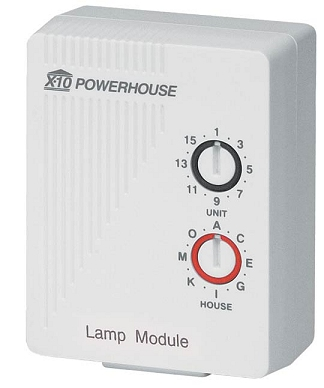
\includegraphics[width=0.15\textwidth]{figs/x10-mod-1}
\hspace{1cm}
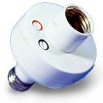
\includegraphics[width=0.15\textwidth]{figs/x10-mod-2}
\caption[Moduli X10]{Esempio di moduli X10 da presa e da porta lampada, Fonte~\cite{smart1}.\label{fig:x10-mod}}
\end{figure}

I dispositivi vengono selezionati attraverso una lettera tra A e P (per l'house code), \tref{tab:x10-table-hcod} e un valore da 1 a 16 (per il key code).
Cambiando il suffisso (ultimo bit del key code) � possibile impostare il comando come mostrato in \tref{tab:x10-table-comcod}.

\begin{table}
\centering
\begin{tabulary}{\textwidth}{CC}
\toprule
\emph{House Code} & \emph{Valore H1-H2-H4-H8} \\\midrule
A & 0110\\
B & 1110\\
C & 0010\\ 
D & 1010\\ 
E & 0001\\ 
F & 1001\\ 
G & 0101\\ 
H & 1101\\ 
I & 0111\\ 
J & 1111\\ 
K & 0011\\ 
L & 1011\\ 
M & 0000\\ 
N & 1000\\ 
O & 0100\\ 
P & 1100\\ 
\bottomrule
\end{tabulary}
\caption[Tabella valori house code protocollo X10]{Valori impostabili dell'House code per ciascun modulo X10.\label{tab:x10-table-hcod}}
\end{table}

\begin{table}
\centering	
\begin{tabulary}{\textwidth}{lClC}
\toprule
\emph{Indirizzo} & \emph{Valore} &\emph{Comando } & \emph{Valore} \\
\emph{Key Code} & \emph{\small D1-D2-D4-D8-D16} & \emph{Key Code} & \emph{\small D1-D2-D4-D8-D16}\\\midrule
1 & 01100 & ON & 00101 \\ 
2 & 11100 & OFF & 00111 \\
3 & 00100 & DIM & 01001 \\ 
4 & 10100 & BRIGHT & 01011 \\ 
5 & 00010 & ALL LIGHTS ON & 00011\\ 
6 & 10010 & ALL UNITS OFF & 00001 \\ 
7 & 01010 & ALL LIGHTS OFF & 01101 \\ 
8 & 11010 & EXTENDED CODE 1 & 01111\\ 
9 & 01110 & HAIL REQUEST & 10001 \\
10& 11110 & HAIL ACK. & 10011 \\ 
11& 00110 & EXTENDED CODE 3& 10101 \\ 
12& 10110 & UNUSED & 10111 \\ 
13& 00000 & EXTENDED CODE 2& 11001 \\ 
14& 10000 & STATUS ``ON'' & 11011 \\
15& 01000 & STATUS ``OFF'' & 11101 \\ 
16& 11000 &	STATUS REQUEST & 11111 \\ 
\bottomrule
\end{tabulary}
\caption[Tabella valori key code protocollo X10]{Valori impostabili di Key Code per ciascun modulo X10.\label{tab:x10-table-comcod}}
\end{table}

%-------------------------------------------------------------------
\subsection{Standard HomePlug}
\label{s:home-dom-lan}
%-------------------------------------------------------------------

Il termine HomePlug indica un protocollo che consente di creare reti telematiche su powerline attraverso i cavi della rete elettrica.
Per poter definire le specifiche e promuovere questo standard � stata creata l'\emph{HomePlug Powerline Alliance}~\cite{hmplug}, un consorzio formato da circa 50 compagnie di settore nato appunto con l'intento di creare un sistema di comunicazione per il \emph{networking domestico} ad alta velocit� tramite powerline.
Esistono due versioni per le reti domestiche: l'HomePlug 1.0 e l'HomePlug AV~\cite{hmover1}.
Il primo consente una velocit� di trasmissione fino a 14 Mbps mentre il secondo, pensato per la TV ad alta definizione e il VOIP consente un massimo bit rate di 200 Mbps\footnote{Ovviamente questi sono tutti valori teorici e dipendono da molti fattori quali per esempio la qualit� dell'impianto elettrico, la struttura, la presenza o meno di fonti di disturbo.}.
Grazie a questi standard � possibile creare delle reti per il collegamento di HDTV, PC, Internet a banda larga in modo semplice e veloce, come mostrato in \fref{fig:hp-ex}.

\afterpage{
\begin{figure}[t]
\centering
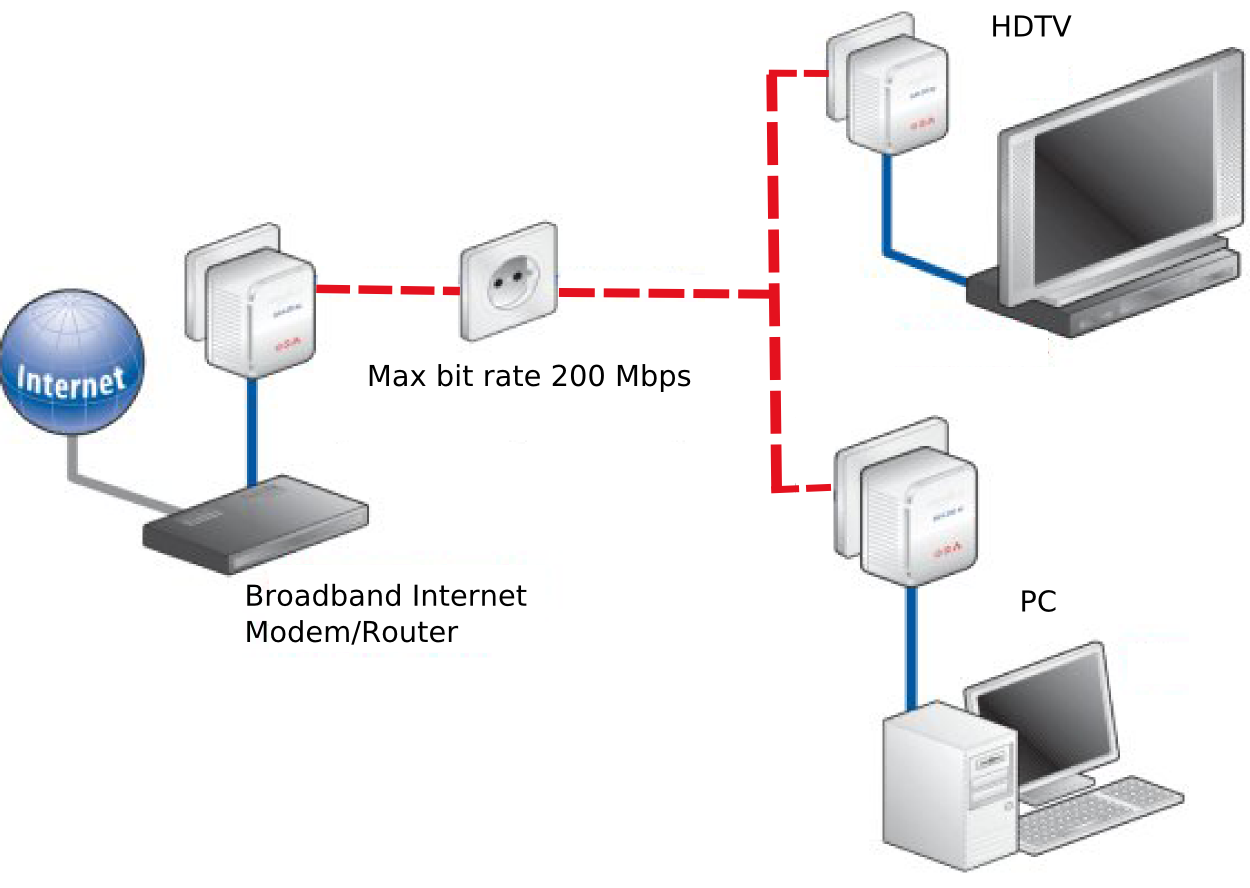
\includegraphics[width=.60\textwidth]{figs/hp-ex}
\caption[Esempio di rete HomePlug]{Esempio di rete HomePlug\footnotemark.\label{fig:hp-ex}}
\end{figure}
\footnotetext{This is a footnote placed within the figure's caption. Notice the use of $\backslash$footnotemark and $\backslash$footnotetext; it is important that $\backslash$footnotetext appears in the same page of $\backslash$footnotemark; this is achieved by the $\backslash$afterpage command.}
}

L'utilizzo della linea elettrica come mezzo fisico per la trasmissione \ac{PLC} risulta molto vantaggiosa grazie alla disponibilit� di prese elettriche in qualunque luogo si possa installare un dispositivo di rete.
Questo porta a diversi vantaggi nell'implementazione di un nuovo concetto di \emph{networking domestico}:

\begin{itemize}
\item facile da installare essendo necessario solo un modulo nella presa elettrica;
\item aumento della sicurezza in quanto i dati viaggiano solo nella rete interna ed in modo crittografato;
\item non sono presenti problemi dovuti a distanze, muri, tubature o qualsiasi altro problema presente con il collegamento wireless;
\item i problemi di interferenze sono risolti attraverso l'impiego della modulazione \ac{ODFM} con 84 possibili frequenze.
\end{itemize}

Una delle principali caratteristiche dell'HomePlug � la sua affidabilit� anche in presenza di interferenze elettromagnetiche.
Le sorgenti di disturbo che potrebbero essere presenti in un abitazione sono: motori e azionamenti elettrici, lampade alogene e fluorescenti, alimentatori, varialuce e antenne radio amatoriali.
Tutto questo introduce notevoli errori sui bit trasmessi, i quali devono in qualche modo essere corretti.
La tecnologia HomePlug utilizza una combinazione di Forward Error Correction \footnote{Parametro che, in una trasmissione digitale, indica quanti dei bit trasmessi sono destinati alla correzione di eventuali errori.} (FEC), Interleaving \footnote{Metodo per l'invio dei messaggi utilizzato nelle reti a pacchetto nelle quali si trasmettono dati non contigui al fine di migliorare le prestazioni in caso di errori.}, riconoscimento degli errori e ripetizione dei dati \ac{ARQ} per poter garantire l'affidabilit� di trasmissione del canale.

Sebbene la comunicazione in una rete HomePlug avvenga soltanto all'interno della rete domestica, quest'ultima � di per se una struttura aperta e per incrementare il livello di sicurezza � stato implementato un sistema di crittografia dei dati.
\`E previsto infatti l'utilizzo a livello MAC della tecnica \ac{DES}\footnote{Algoritmo di cifratura basato su chiave a 56 bit.}.
Inoltre i dispositivi su una stessa rete condividono la stessa chiave per la quale � previsto anche un sistema di distribuzione tra i nodi.

%-------------------------------------------------------------------
\subsection{Protocollo PowerDom}
\label{s:powerdom-dom-lan}
%-------------------------------------------------------------------

Il PowerDom~\cite{powdom} � un sistema domotico di nuova concezione in grado di realizzare una rete domestica sulle linee di alimentazione 220V, comunemente disponibili all'interno delle abitazioni.
La realizzazione, come da caratteristica di un sistema powerline, non richiede una particolare infrastruttura ad hoc e nemmeno la posa di nuovi cavi, ma richiede semplicemente di poter accedere all'impianto elettrico per l'installazione dei relativi moduli.
I moduli comunicano attraverso una \ac{PLC} con portante multifrequenza variabile tra 60 Khz e 132 Khz con modulazione \ac{FSK}.
Il massimo bit rate di trasmissione � di 4800 bps.
Attraverso l'impiego di una o pi� centrali di controllo touch screen (PowerGuard) � possibile comandare e configurare diversi dispositivi come:

\begin{itemize}
\item moduli di allarme (PowerEye);
\item moduli per la segnalazione acustica (PowerAlarm);
\item moduli per il controllo degli accessi (PowerAccess);
\item moduli per il controllo delle utenze (PowerControl);
\item moduli per il controllo del riscaldamento e climatizzazione (PowerClima);
\end{itemize}

La vera novit� del sistema PowerDom � l'uso intensivo del controllo remoto delle funzioni principali.
Attraverso un software installabile su tutti i pi� comuni smartphone, \fref{fig:powerdom-sms}, � possibile mantenere sotto controllo la propria abitazione.
Il programma permette per esempio di attivare e disattivare gli allarmi, accendere e spegnere le utente.
Inoltre il sistema autonomamente provvede a inviare un SMS nel caso in cui si verifichino accessi non autorizzati, malfunzionamenti o allarmi diversi.

\begin{figure}[t]
\centering
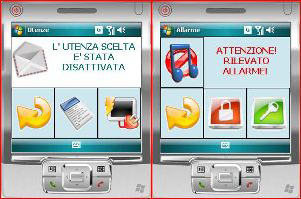
\includegraphics[width=.40\textwidth]{figs/powerdom-sms}
\caption[Software smartphone PowerDom]{Software smartphone PowerDom. Fonte:~\cite{powdom}\label{fig:powerdom-sms}}
\end{figure}

%-------------------------------------------------------------------
\section{Internet a banda larga}
\label{s:broadband}
%-------------------------------------------------------------------

Un altro possibile impiego per il quale la tecnologia powerline pu� essere una ottima soluzione � quello della diffusione di Internet a banda larga, mediante il cosiddetto \ac{BPLC}.
La \ac{BPLC} viene utilizzata per quei luoghi, non coperti dal normale servizio ADSL e per i quali a causa di condizioni territoriali sfavorevoli, come la presenza di alberi, montagne o altri ostacoli, non � possibile impiegare direttamente la tecnologia wireless.
Anche laddove fosse possibile installare un ripetitore wi-fi ma le utenze richieste non siano sufficienti a coprire le spese per posizionare il ripetitore ad un altezza tale da coprire la zona, viene utilizzata una soluzione ibrida composta dal segnale wireless pi� la trasmissione su powerline.
In questi casi risulta quindi pi� comodo e meno costoso collegare un convertitore che invia il segnale sul cavo elettrico, partendo dal ripetitore wireless pi� vicino.
Oltre al vantaggio di riuscire a collegare anche le utenze pi� difficili, � probabile infatti che sia sempre presente un cavo elettrico su cui poter trasmettere, si ottiene un sensibile risparmio di cablaggio in fibra delle centraline a bassa tensione\footnote{Centrali elettriche a cui fanno capo tutte le abitazioni che sono a loro volta collegate a quelle di media tensione.}.
A queste ultime la banda larga pu� essere inviata per esempio tramite i meno costosi ponti radio.
Inoltre attraverso l'utilizzo del segnale wireless � possibile mantenere una qualit� migliore e latenze pi� basse anche su notevoli distanze rispetto all'utilizzo del cavo in rame, a patto che siano attuati i corretti meccanismi sui nodi trasmettitori (es. algoritmi di correzione del segnale).
In \fref{fig:plc-wifi} � mostrato un esempio della rete ibrida.

\begin{figure}
\centering
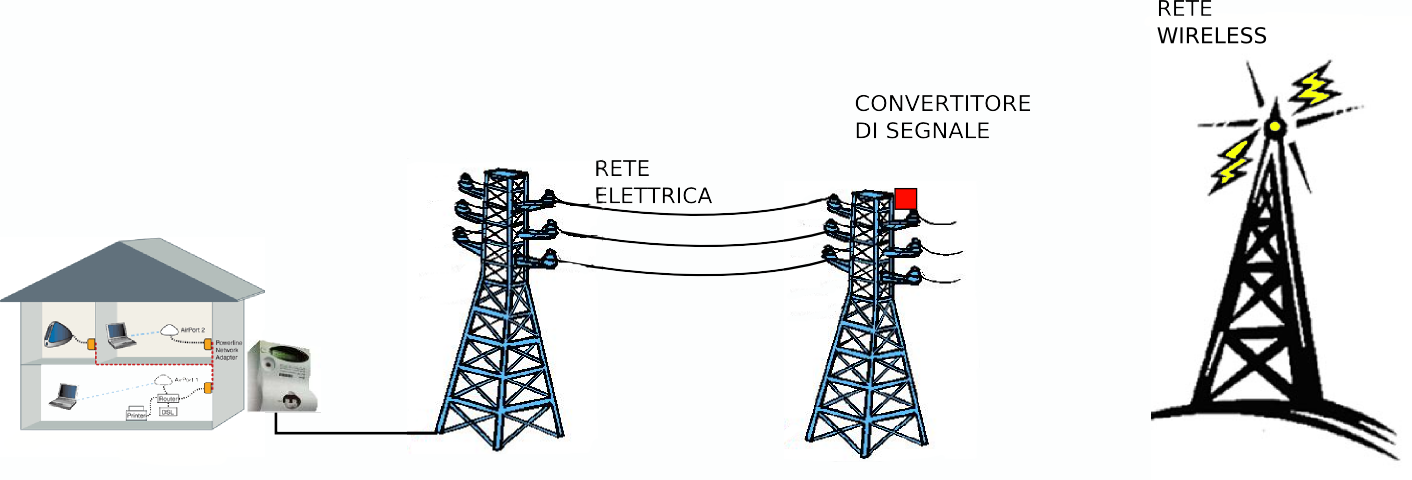
\includegraphics[width=.80\textwidth]{figs/plc-wifi}
\caption[Esempio rete ibrida Wifi-powerline]{Esempio rete ibrida Wifi-powerline.\label{fig:plc-wifi}}
\end{figure}

Un progetto di questo tipo, nel quale per� la connessione ad internet della cabina elettrica � effettuato in fibra ottica, � stato realizzato a Brescia~\cite{plcbs1}.

%-------------------------------------------------------------------
\section{Applicazioni automotive}
\label{s:automotive}
%-------------------------------------------------------------------

I vantaggi derivanti dall'utilizzo della tecnologia powerline possono essere trasferiti anche in ambito Automotive, come descritto nella \sref{s:com-auto}.
Esistono dei prototipi di modem transceiver che consentono di implementare una comunicazione powerline andando a sostituire il livello fisico dei gi� affermati bus \ac{CAN} e \ac{LIN} operanti su linea dedicata.
I componenti che verranno considerati, prodotti dalla \emph{Yamar Electronics Ltd}\footnote{\url{http://www.yamar.com}}, sono i seguenti: DCAN250, \sref{sc:dcan250-automotive} e SIG40, \sref{sc:sig40-automotive}.

Per un possibile impiego di questi componenti e soluzioni � comunque fondamentale assicurarsi che essi forniscano delle prestazioni minime, in termini di bit rate, almeno comparabili con quelle del \ac{CAN} e \ac{LIN}.
Da questo punto di vista i primi componenti citati, risultano a prestazioni ridotte rispetto a quelle fornite dal diffusissimo CAN.
L'unico componente in grado di offrire prestazioni paragonabili � il DCB500, prodotto sempre da Yamar Electronics Ltd, che sar� considerato e descritto meglio nella \sref{s:comp-trasm-dcb500}.

Dato che attualmente le prestazioni del diffusissimo e affermatissimo \ac{CAN} bus sono molto al di sopra di quelle possibili con questi due dispositivi, si � deciso di impiegare, per lo sviluppo di questa tesi, un altro dispositivo che consente di unire le potenzialit� di una comunicazione su DC-BUS\footnote{Digital Current - Bus, bus a tensione continua.} al mantenimento di un bit rate di comunicazione idoneo alle applicazioni automotive.
Il dispositivo menzionato � il DCB500 di cui si parler� nella \sref{s:comp-trasm-dcb500}.

%-------------------------------------------------------------------
\subsection{DCAN250}
\label{s:dcan250-automotive}
%-------------------------------------------------------------------

Il DCAN250~\cite{dcan250} � un dispositivo che consente di sostituire il livello fisico del \ac{CAN} bus e poter utilizzare una powerline come linea di comunicazione.
Si comporta come un vero e proprio \emph{transceiver} e consente di collegare tutti quei dispositivi che fanno uso del protocollo \ac{CAN}: dal controllo del volante, alle portiere, sensori, display, pannelli di controllo, ecc.
Il DCAN250 contiene al suo interno un modem, un codificatore/decodificatore per il canale, un communication controller e un buffer per i dati che devono essere inviati sul bus.
Come tutti i dispositivi basati sulla tecnologia DC-BUS consente di ridurre il complesso cablaggio all'interno del veicolo e fornisce una facile e veloce installazione.

Il segnale viene modulato con la tecnica DQPSK e sono implementati anche protocolli di risoluzione delle collisioni, correzione degli errori e risparmio energetico (Modalit� \emph{sleep} per i nodi in stand-by).
Fra le caratteristiche di questo dispositivo vi � la possibilit� di connettere allo stesso \dcbus\ fino a 16 nodi, che comunicano tra loro utilizzando l'affidabile protocollo \ac{CAN} attraverso una powerline. 

%-------------------------------------------------------------------
\subsection{SIG40}
\label{s:sig40-automotive}
%-------------------------------------------------------------------

Anche il SIG40~\cite{sig40} � un transceiver che consente di realizzare una comunicazione digitale su powerline eliminando i collegamenti altrimenti necessari per il controllo e per i dati.
Si propone come sostituto del livello fisico di UART e \ac{LIN}.
Pu� essere impiegato in svariati ambiti dall'automotive, all'avionica e all'industria.
Applicazioni tipiche possono essere: la lettura di sensori, attivazione di attuatori, controllo di porte, specchietti, condizionamento, luci e molto altro.
Al suo interno contiene un modem, un'interfaccia di collegamento all'host, driver e filtri.
Se impiegato come sostituto del livello fisico del \ac{LIN} consente di triplicarne la velocit� fino ad un bit rate massimo di 57.6 Kbps.
Sullo stesso \dcbus\ possono inoltre essere presenti diverse sottoreti che trasmettono ciascuna con una frequenza della portante diversa (4.5-6.5 Mhz).
Il SIG40 pu� inoltre essere integrato in una qualsiasi applicazione CMOS come per esempio un microcontrollore.


%-------------------------------------------------------------------
\chapter{Conclusions}
\label{c:conc}
%-------------------------------------------------------------------

\epigraph{``Computer Science is no more about computers than astronomy is about telescopes.''}{\emph{E. W. Dijkstra}}

Lorem ipsum dolor sit amet, consectetur adipiscing elit, sed do eiusmod tempor incididunt ut labore et dolore magna aliqua.
Ut enim ad minim veniam, quis nostrud exercitation ullamco laboris nisi ut aliquip ex ea commodo consequat.
Duis aute irure dolor in reprehenderit in voluptate velit esse cillum dolore eu fugiat nulla pariatur.
Excepteur sint occaecat cupidatat non proident, sunt in culpa qui officia deserunt mollit anim id est laborum.


%\backmatter

%-------------------------------------------------------------------
% Bibliography
%-------------------------------------------------------------------
\label{Bibliography}
\bibliographystyle{plain}
\bibliography{biblio}

\end{document}
